\documentclass[
11pt, % The default document font size, options: 10pt, 11pt, 12pt
%codirector, % Uncomment to add a codirector to the title page
]{charter} 


% El títulos de la memoria, se usa en la carátula y se puede usar el cualquier lugar del documento con el comando \ttitle
\titulo{Videojuego portátil inspirado en consolas retro} 

% Nombre del posgrado, se usa en la carátula y se puede usar el cualquier lugar del documento con el comando \degreename
\posgrado{Carrera de Especialización en Sistemas Embebidos} 
%\posgrado{Carrera de Especialización en Internet de las Cosas} 
%\posgrado{Carrera de Especialización en Inteligencia Artificial}
%\posgrado{Maestría en Sistemas Embebidos} 
%\posgrado{Maestría en Internet de las cosas}

% Tu nombre, se puede usar el cualquier lugar del documento con el comando \authorname
% IMPORTANTE: no omitir titulaciones ni tildación en los nombres, también se recomienda escribir los nombres completos (tal cual los tienen en su documento)
\autor{Lic. Jezabel Victoria Danon}

% El nombre del director y co-director, se puede usar el cualquier lugar del documento con el comando \supname y \cosupname y \pertesupname y \pertecosupname
\director{Título y Nombre del director}
\pertenenciaDirector{pertenencia} 
\codirector{} % para que aparezca en la portada se debe descomentar la opción codirector en los parámetros de documentclass
\pertenenciaCoDirector{FIUBA}

% Nombre del cliente, quien va a aprobar los resultados del proyecto, se puede usar con el comando \clientename y \empclientename
\cliente{Lic. Jezabel Victoria Danon}
\empresaCliente{Proyecto personal}
 
\fechaINICIO{29 de abril de 2025}		%Fecha de inicio de la cursada de GdP \fechaInicioName
\fechaFINALPlan{18 de junio de 2025} 	%Fecha de final de cursada de GdP
\fechaFINALTrabajo{15 de diciembre de 2025}	%Fecha de defensa pública del trabajo final


\begin{document}

\maketitle
\thispagestyle{empty}
\pagebreak


\thispagestyle{empty}
{\setlength{\parskip}{0pt}
\tableofcontents{}
}
\pagebreak


\section*{Registros de cambios}
\label{sec:registro}


\begin{table}[ht]
\label{tab:registro}
\centering
\begin{tabularx}{\linewidth}{@{}|c|X|c|@{}}
\hline
\rowcolor[HTML]{C0C0C0} 
Revisión & \multicolumn{1}{c|}{\cellcolor[HTML]{C0C0C0}Detalles de los cambios realizados} & Fecha      \\ \hline
0      & Creación del documento                                 &\fechaInicioName \\ \hline
1      & Se completa hasta el punto 5 inclusive                & {10} de {mayo} de 2025 \\ \hline
2      & Se completa hasta el punto 9 inclusive \newline
		  Agrega usuario final \newline
		  Cambio de cliente \newline
		  Cambio de título del proyecto                    & {19} de {mayo} de 2025 \\ \hline
%3      & Se completa hasta el punto 12 inclusive                & {día} de {mes} de 202X \\ \hline
%4      & Se completa el plan	                                 & {día} de {mes} de 202X \\ \hline

% Si hay más correcciones pasada la versión 4 también se deben especificar acá

\end{tabularx}
\end{table}

\pagebreak



\section*{Acta de constitución del proyecto}
\label{sec:acta}

\begin{flushright}
Buenos Aires, \fechaInicioName
\end{flushright}

\vspace{2cm}

Por medio de la presente se acuerda con la \authorname\hspace{1px} que su Trabajo Final de la \degreename\hspace{1px} se titulará ``\ttitle'' y consistirá en 
%\textcolor{red}{la implementación de un prototipo de un sistema de control de temperatura de una caldera industrial}. 
el desarrollo de un prototipo de consola de videojuegos portátil minimalista con un único juego integrado. 
El trabajo tendrá un presupuesto preliminar estimado de 
720 horas y un costo estimado de 
%\textcolor{red}{\$ XXX}, 
€ 120 (ciento veinte euros),
con fecha de inicio el \fechaInicioName\hspace{1px} y fecha de presentación pública el \fechaFinalName.

Se adjunta a esta acta la planificación inicial.

\vfill

% Esta parte se construye sola con la información que hayan cargado en el preámbulo del documento y no debe modificarla
\begin{table}[ht]
\centering
\begin{tabular}{ccc}
\begin{tabular}[c]{@{}c@{}}Dr. Ing. Ariel Lutenberg \\ Director posgrado FIUBA\end{tabular} & \hspace{2cm} & \begin{tabular}[c]{@{}c@{}}\clientename \\ \empclientename \end{tabular} \vspace{2.5cm} \\ 
\multicolumn{3}{c}{\begin{tabular}[c]{@{}c@{}} \supname \\ Director del Trabajo Final\end{tabular}} \vspace{2.5cm} \\
\end{tabular}
\end{table}




\section{1. Descripción técnica-conceptual del proyecto a realizar}
\label{sec:descripcion}

%{Cubre: contexto y objetivos y problema}
El proyecto responde a una temática de interés personal y tiene como objetivo principal acreditar los conocimientos obtenidos en el postgrado. Esto implica la utilización de diversos módulos de hardware y la implementación de técnicas de ingeniería de software específicas para sistemas embebidos. Como objetivo secundario, se planteó que el área de aplicación seleccionada no requiriera del asesoramiento experto de terceros, para maximizar el enfoque en el uso autónomo de los contenidos de la carrera de especialización. También se consideró que el proyecto fuera viable para alguien sin experiencia previa en estos temas.

%{solución}
La solución propuesta es un sistema embebido que articula los conocimientos del posgrado, manteniendo una complejidad técnica abordable. El desarrollo incluye el uso coordinado de periféricos variados y protocolos de comunicación comunes en sistemas reales. Además, requiere diseñar una arquitectura de software clara, con módulos separados para entrada, salida y lógica de control del sistema. La aplicación final consiste en una consola de videojuegos portátil inspirada en dispositivos retro, con algunas mejoras funcionales propias de plataformas actuales.

%{estado del arte}
Las primeras consolas portátiles de videojuegos, conocidas como \textit{handheld consoles}, establecieron una lógica de diseño centrada en la simplicidad, la portabilidad y el uso eficiente de recursos. Dispositivos como Mattel Auto Race (1976) o Electronic Football (1977) usaban pantallas de LED y una mecánica de juego muy básica, basada en puntos luminosos. Más adelante, la serie Game \& Watch (Nintendo, 1980) introdujo pantallas LCD y juegos integrados en hardware dedicado. La aparición de consolas como la Game Boy (Nintendo), la Atari Lynx y la Sega Game Gear, entre 1989 y 1990, permitió expandir estas ideas mediante cartuchos intercambiables, mayor calidad gráfica y audio mejorado, sin abandonar el enfoque de sistema cerrado y orientado exclusivamente al juego. Estas plataformas funcionaban con microprocesadores de 4, 8 o hasta 16 bits, sin sistemas operativos ni procesamiento paralelo, y su interacción se limitaba a botones físicos y salidas visuales y sonoras básicas.

Con el tiempo, las consolas \textit{handheld} evolucionaron hacia arquitecturas más complejas, con mejores capacidades gráficas, pantallas retroiluminadas a color, sonido estéreo y almacenamiento digital. También incorporaron nuevas formas de interacción, como pantallas táctiles, sensores de movimiento y motores de vibración. Estas incorporaciones permitieron enriquecer la experiencia de juego sin perder la portabilidad ni la simplicidad de uso. Aunque no todas estas tecnologías se consolidaron como estándar en el ámbito portátil, abrieron nuevas posibilidades para la interacción física y sensorial entre el usuario y el dispositivo.


%{descripción funcional}
El sistema a desarrollar adoptará una arquitectura cerrada y específica, centrada en la ejecución de un único videojuego implementado directamente en el firmware del dispositivo. Al iniciarse, el juego permitirá controlar la simulación del vuelo de una aeronave a partir de la interacción con botones y un joystick analógico, los cuales enviarán señales al sistema en tiempo real. La respuesta del sistema se manifestará a través de una interfaz visual, junto con retroalimentación sonora y háptica asociada a distintos eventos del juego.

El prototipo incluirá sensores de movimiento que permitirán detectar variaciones de posición del dispositivo. La información capturada del sensor, los botones y el joystick será procesada para determinar parámetros de vuelo tales como velocidad, altitud, dirección y posición de la aeronave dentro de un mapa predefinido. Dichos parámetros permitirán actualizar la representación gráfica, sonora y táctil de la simulación. 

En la figura \ref{fig:diagBloques} se presenta el diagrama en bloques del sistema, en el que se observa el microcontrolador que coordinará el funcionamiento de los distintos módulos: entradas (botones, joystick, sensores), salidas (pantalla, audio, vibración) y almacenamiento externo. El estado del juego deberá guardarse en memoria no volátil, utilizando una EEPROM externa o una tarjeta SD, permitiendo su recuperación tras un reinicio. El prototipo se conectará a una fuente de alimentación portátil.

%{diagrama de bloques}
\begin{figure}[htpb]
\centering 
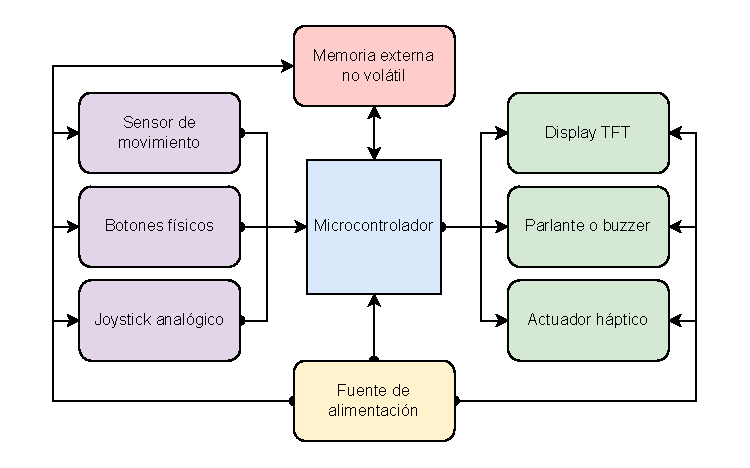
\includegraphics[width=.85\textwidth]{./Figuras/diagrama_bloques_proyecto.pdf}
\caption{Diagrama en bloques del sistema.}
\label{fig:diagBloques}
\end{figure}

\vspace{25px}

%{propuesta de valor}
El presente proyecto no se plantea como un producto de innovación con proyección comercial, pero se distingue por reinterpretar el concepto de consola portátil clásica desde una perspectiva actual. A partir de una arquitectura simple y dedicada, centrada en un único juego, se incorporan características técnicas poco comunes en dispositivos de este tipo, como el uso de un microcontrolador de 32 bits, pantalla a color, sensores de movimiento, retroalimentación háptica y almacenamiento persistente del estado del juego.



% \begin{consigna}{red} % ELIMINAR \begin{consigna}{red} y \end{consigna}{red} en las secciones que vayan completando para cada entrega parcial.
% El objetivo es que el lector, en una o dos páginas, exponga de qué se trata el proyecto y cuáles son sus desafíos, cuál es la motivación para realizarlo y su importancia.

% Se debe introducir el contexto del proyecto, el estado del arte en la temática, describir la propuesta de valor, cuál es el problema que atiende y cuál es la solución que se propone. Se debe dar una descripción funcional de la solución que incluya un diagrama en bloques.

% Puede ser útil incluir en esta sección la respuesta a alguna de estas preguntas:

% \begin{itemize}
% 	\item ¿Cuál es el contexto del proyecto, es un emprendimiento personal, un proyecto para una empresa, es parte del programa de vinculación con empresas del posgrado?
% 	\item ¿Existen o aplican condiciones especiales al proyecto, financiamiento de algún programa público o privado, acuerdos de confidencialidad, acuerdos sobre la propiedad intelectual de los entregables u otros?
% 	\item ¿Cómo se compara la solución propuesta con el estado del arte en el campo de aplicación? ¿En qué aspectos destaca?
% 	\item ¿Ayuda a la explicación si se incluye un lienzo Canvas del Modelo de Negocio?
% 	\item ¿En qué estado del ciclo de vida está la solución que se propone?
% 	\item ¿Cuáles son las características del cliente (el adoptante de los entregables del proyecto) qué valora, qué necesita?
% 	\item ¿Por dónde pasa la innovación?
% \end{itemize}

% La descripción técnica-conceptual \textbf{debe incluir al menos un diagrama en bloques del sistema} y descripción funcional de la solución propuesta.

% Las figuras se deben mencionar en el texto ANTES de que aparezcan con una frase como la siguiente: ``En la figura \ref{fig:diagBloques} se presenta el diagrama en bloques del sistema. Se observa que...''.  La regla es que las figuras nunca pueden ir antes de ser mencionadas en el texto, porque sino el lector no entiende por qué de pronto aparece una figura.

% \begin{figure}[htpb]
% \centering 
% \includegraphics[width=.65\textwidth]{./Figuras/diagBloques.png}
% \caption{Diagrama en bloques del sistema.}
% \label{fig:diagBloques}
% \end{figure}

% \vspace{25px}

% El tamaño del texto en TODAS las figuras debe ser adecuado \textbf{para que NO pase lo que ocurre en la figura \ref{fig:diagBloques}}, donde el lector debe esforzarse para poder leer el texto. 

% Los colores usados en el diagrama deben ser adecuados, tal que ayuden a comprender mejor el diagrama. Se recomienda evitar colores primarios (como rojo, verde o cyan) y usar la gama de colores pastel.

% \end{consigna} % ELIMINAR \begin{consigna}{red} y \end{consigna}{red} en las secciones que vayan completando para cada entrega parcial.

\section{2. Identificación y análisis de los interesados}
\label{sec:interesados}

% \begin{consigna}{red} % ELIMINAR \begin{consigna}{red} y \end{consigna}{red} en las secciones que vayan completando para cada entrega parcial.
% \textbf{Nota importante:} borrar esto y todas las consignas en color rojo antes de entregar este documento). Esto se hace eliminando el par de comandos que forman el bloque consigna, \verb!\begin{consigna}{red}! y \verb!\end{consigna}{red}! del código. 
 
% Es inusual que una misma persona esté en más de un rol, incluso en proyectos chicos. Si se considera que una persona cumple dos o más roles, entonces \textbf{solo dejarla en el rol más importante}. 

% Por ejemplo, si una persona es Cliente pero también colabora u orienta, dejarla solo como Cliente. Si una persona es el Responsable, \textbf{no debe ser colocado también como miembro del equipo}.


\begin{table}[ht]
%\caption{Identificación de los interesados}
%\label{tab:interesados}
\begin{tabularx}{\linewidth}{@{}|l|L{4.7cm}|X|l|@{}}
\hline
\rowcolor[HTML]{C0C0C0} 
Rol           & Nombre y Apellido & Organización 	& Puesto 	\\ \hline
%Auspiciante   & \authorname     &  FIUBA        	&  -      	\\ \hline
Cliente       & \clientename      &\empclientename	&       	\\ \hline
%Impulsor      &                   &              	&        	\\ \hline
Responsable   & \authorname       & FIUBA        	& Alumno 	\\ \hline
%Colaboradores &                   &              	&        	\\ \hline
Orientador    & \supname	      & \pertesupname 	& Director del Trabajo Final \\ \hline
%Equipo        & miembro1 \newline 
%				miembro2          &              	&        	\\ \hline
%Opositores    &                   &              	&        	\\ \hline
Usuario final &  Entusiastas de sistemas embebidos o videojuegos retro &   	&   	\\ \hline
\end{tabularx}
\end{table}

\begin{itemize}
	\item Cliente: al tratarse de un proyecto académico, se utilizará la figura de cliente a nombre del autor y responsable.
	\item Responsable: será el autor del presente documento, encargado del desarrollo del prototipo y del cumplimiento de los requerimientos pautados en la planificación.
	\item Usuario final: personas con conocimientos técnicos básicos o intermedios, interesados en sistemas embebidos y/o videojuegos retro. 
\end{itemize}
% El Director suele ser uno de los orientadores.

% No dejar celdas vacías; si no hay nada que poner en una celda colocar un signo ``-''.

% No dejar filas vacías; si no hay nada que poner en una fila entonces eliminarla.

% Es deseable listar a continuación las principales características de cada interesado.
 
% Por ejemplo:
% \begin{itemize}
% 	\item Orientador: la Dra. Ing. María Gómez es experta en la temática y va a ayudar con la definición de los requerimientos y el desarrollo del firmware del embebido.
% 	\item Auspiciante: es riguroso y exigente con la rendición de gastos. Tener mucho cuidado con esto.
% 	\item Equipo: Juan Perez, suele pedir licencia porque tiene un familiar con una enfermedad. Planificar considerando esto.
% \end{itemize}

% \end{consigna} % ELIMINAR \begin{consigna}{red} y \end{consigna}{red} en las secciones que vayan completando para cada entrega parcial.


\section{3. Propósito del proyecto}
\label{sec:proposito}

Aplicar de forma integrada los conocimientos adquiridos durante el posgrado en una solución técnica concreta, desarrollada de manera autónoma. Se busca abordar un caso representativo de sistemas embebidos que permita ejercitar competencias clave de la carrera, como la gestión de periféricos, la programación en tiempo real y el diseño modular de software. 

% \begin{consigna}{red} % ELIMINAR \begin{consigna}{red} y \end{consigna}{red} en las secciones que vayan completando para cada entrega parcial.

% ¿Por qué se hace el proyecto? ¿Qué se quiere lograr? 

% Se recomienda que sea solo un párrafo que continúe con la idea de la frase ``el propósito de este proyecto es...'' (omitir la frase, ya que está en el título de la sección).
% \end{consigna}

\section{4. Alcance del proyecto}
\label{sec:alcance}

% \begin{consigna}{red}
% ¿Qué se incluye y que no se incluye en este proyecto?

% Se refiere al trabajo que se va a hacer para entregar el producto o resultado especificado. 

% Explicitar todo lo quede comprendido dentro del alcance del proyecto. Por ejemplo:

El proyecto incluye:
\begin{itemize}
	\item El diseño y construcción de un prototipo funcional de consola portátil de videojuegos.
	\item El desarrollo de un juego de simulación de vuelo, implementado directamente en el firmware.
	\item La integración de periféricos de entrada:
		\begin{itemize}
		\item Botones físicos.
		\item Joystick analógico.
		\item Sensor de movimiento (acelerómetro y/o giroscopio).
		\end{itemize}
	\item La integración de periféricos de salida:
		\begin{itemize}
		\item Pantalla TFT (a color).
		\item Salida sonora mediante parlante o buzzer.
		\item Motor de vibración para retroalimentación háptica.
		\end{itemize}
	\item El almacenamiento del estado del juego en memoria no volátil.
	\item La documentación técnica requerida para su presentación como trabajo final de especialización.
\end{itemize}
El presente proyecto no incluye:
\begin{itemize}
	\item El diseño y/o la fabricación de una placa de circuito impreso (PCB, por \textit{Printed Circuit Board}).
	\item El desarrollo de un entorno ejecutable separado del juego: el firmware no estará diseñado de forma general para admitir juegos en formatos estándar.
	\item Conectividad externa, comunicación inalámbrica o funcionalidades multijugador.
\end{itemize}
% Explicitar además todo lo que no quede incluido (``El presente proyecto no incluye...'')

% \end{consigna} % ELIMINAR \begin{consigna}{red} y \end{consigna}{red} en las secciones que vayan completando para cada entrega parcial.


\section{5. Supuestos del proyecto}
\label{sec:supuestos}

%\begin{consigna}{red} % ELIMINAR \begin{consigna}{red} y \end{consigna}{red} en las secciones que vayan completando para cada entrega parcial.
Para el desarrollo del presente proyecto se supone que: 

\begin{itemize}
	\item Se dispondrá de los materiales y componentes necesarios para el prototipo funcional.
	\item Las horas estimadas de trabajo serán suficientes para cumplir con los objetivos planteados.
	\item Los conocimientos requeridos para avanzar en las distintas etapas del proyecto se alcanzarán durante el transcurso del posgrado en tiempos compatibles con el desarrollo.
	\item La solución planteada es técnicamente viable dentro del alcance y recursos definidos.
	\item El responsable dispondrá de dedicación a tiempo completo hasta culminar el proyecto.
\end{itemize}

% Por ejemplo, se podrían incluir supuestos respecto a disponibilidad de tiempo y recursos humanos y materiales, sobre la factibilidad técnica de distintos aspectos del proyecto, sobre otras cuestiones que sean necesarias para el éxito del proyecto como condiciones macroeconómicas o reglamentarias.

%\end{consigna} % ELIMINAR \begin{consigna}{red} y \end{consigna}{red} en las secciones que vayan completando para cada entrega parcial.

\section{6. Requerimientos}
\label{sec:requerimientos}

Los requerimientos del proyecto son los siguientes:

\begin{enumerate}
	\item Requerimientos de hardware:
	\begin{enumerate}
		\item El prototipo deberá montarse en \textit{protoboard} o soldarse sobre placas de experimentación.
		\item El prototipo deberá alimentarse a través de una batería.
		\item El prototipo deberá integrar un sensor capaz de medir la inclinación en al menos dos ejes.
		\item El prototipo deberá integrar un joystick analógico con capacidad de lectura en dos ejes.
		\item El prototipo deberá incluir botones tipo switch para funciones definidas.
		\item El prototipo deberá incorporar una pantalla capaz de mostrar información visual relevante para el juego.
		\item El prototipo deberá incluir un mecanismo para emitir sonidos o alertas sonoras.
		\item El prototipo deberá integrar un motor de vibración capaz de generar retroalimentación háptica.
		\item El prototipo deberá contar con memoria no volátil para el almacenamiento persistente del estado del juego.
	\end{enumerate}
	\item Requerimientos de firmware:
	\begin{enumerate}
		\item El firmware deberá implementar la lógica para interpretar los datos del sensor de inclinación y el joystick para controlar el modelo de vuelo (cabeceo, alabeo, giro, velocidad).
		\item El firmware deberá incluir un demo de juego integrado que permita demostrar la lógica implementada y la funcionalidad de los periféricos de entrada y salida.
		\item El firmware deberá gestionar la visualización de la información del juego en la pantalla.
		\item El firmware deberá ser capaz de reproducir las alertas sonoras necesarias.
		\item El firmware deberá controlar la activación y duración del motor de vibración en función de los eventos del juego.
		\item El firmware deberá implementar la lógica para guardar y cargar el estado del juego en la memoria no volátil.
		\item El firmware deberá detectar las pulsaciones de los botones y activar las funcionalidades correspondientes (inicio/fin, pausa, guardar, mapa, etc...).
	\end{enumerate}
	\item Requerimientos de documentación:
	\begin{enumerate}
		\item Diagrama de conexión de módulos.
		\item Video demostrativo del uso de las funcionalidades requeridas.
		\item Informe de avance.
		\item Memoria técnica.
	\end{enumerate}
	\item Requerimientos opcionales:
	\begin{enumerate}
		% \item El firmware podrá utilizar un sistema operativo de tiempo real (RTOS por sus siglas en inglés) para gestionar tareas concurrentes como lectura de sensores y salida de señales.
		\item El firmware podrá incluir gráficos a color para representar la interfaz de usuario (UI por sus siglas en inglés).
		\item El sistema podrá incluir uno o varios selectores de niveles para aspectos como: el volumen de las señales audio, el nivel de vibración de la consola, modos de visualización diferentes para debug o gráficos, entre otras opciones posibles.
	\end{enumerate}
\end{enumerate}

\section{7. Historias de usuarios (\textit{Product backlog})}
\label{sec:backlog}

Escalas utilizadas para asignar \textit{story points}:
\begin{enumerate}
	\item Complejidad:
	\begin{itemize}
		\item Baja complejidad: 1 Punto
		\item Media complejidad: 3 Puntos
		\item Alta complejidad: 5 Puntos
	\end{itemize}
	\item Cantidad de trabajo:
	\begin{itemize}
		\item Poco trabajo: 1 Punto
		\item Cantidad de trabajo media: 2 Puntos
		\item Mucho trabajo: 3 Puntos
	\end{itemize}
	\item Incertidumbre asociada:
	\begin{itemize}
		\item  Baja incertidumbre: 2 Puntos
		\item  Incertidumbre media: 5 Puntos
		\item  Alta incertidumbre: 8 Puntos
	\end{itemize}
\end{enumerate}

\textbf{Épica 1:} Control e interacción del usuario con el demo de juego

	\textbf{HU1: Control intuitivo por inclinación.} Como usuario, quiero controlar el cabeceo (\textit{pitch}) y el alabeo (\textit{roll}) de la aeronave inclinando la consola, para tener una experiencia de control más natural e inmersiva.

	Criterios de aceptación:
	\begin{itemize}
		\item El sistema interpreta la inclinación de la consola en los ejes X e Y como comandos de alabeo y cabeceo respectivamente.
		\item La respuesta del modelo de vuelo a la inclinación es inmediata y fluida, sin latencia perceptible.
		\item El control debe estar calibrado en un rango usable (sin saturar los extremos).
		\item Se pueden realizar movimientos suaves y precisos con pequeñas inclinaciones.
	\end{itemize}
	\textit{Story points}: 13 (complejidad: 3, trabajo: 2, incertidumbre: 5)

	\textbf{HU2: Maniobras precisas con el joystick.} Como usuario, quiero usar el joystick analógico para controlar el giro (\textit{yaw}) y la velocidad de la aeronave, para poder realizar maniobras precisas y ajustar mi trayectoria.

	Criterios de aceptación:
	\begin{itemize}
		\item El movimiento horizontal del joystick controla el ángulo de giro de la aeronave de forma proporcional.
		\item El movimiento vertical del joystick controla la velocidad de avance de la aeronave.
		\item El control de giro es suave y permite realizar ajustes finos.
	\end{itemize}
	\textit{Story points}: 8 (complejidad: 3, trabajo: 2, incertidumbre: 2)
		
	\textbf{HU3: Inicio y fin de sesión sencillos.} Como usuario, quiero poder iniciar el juego rápidamente al encender la consola y finalizarla fácilmente cuando termine de jugar.

	Criterios de aceptación:
	\begin{itemize}
		\item Al presionar el botón de ``Inicio", la demostración del juego comienza en un estado predefinido.
		\item Al presionar el botón de ``Finalizar", el juego se detiene y la consola vuelve a un menú principal o estado de espera.
	\end{itemize}
	\textit{Story points}: 5 (complejidad: 1, trabajo: 1, incertidumbre: 2)
		
\textbf{Épica 2:} Visualización del entorno y mapa

	\textbf{HU4: Información clara del estado.} Como usuario, quiero ver en pantalla información clave como mi velocidad, dirección y posición, para estar siempre informado sobre el estado de mi juego.

	Criterios de aceptación:
	\begin{itemize}
		\item La velocidad, dirección y posición actual de la aeronave se representan visualmente en la pantalla.
		\item Los cambios en la velocidad, dirección y posición se reflejan en la pantalla en tiempo real (sin lags perceptibles).
	\end{itemize}
	\textit{Story points}: 21 (complejidad: 5, trabajo: 2, incertidumbre: 8)
		
	\textbf{HU5: Visualizar ubicación en el mapa.} Como usuario, quiero ver la posición actual de la aeronave en el mapa, para tener una referencia de navegación.

	Criterios de aceptación:
	\begin{itemize}
		\item Al presionar el botón de ``Mapa", se muestra una representación del entorno de vuelo.
		\item La posición actual de la aeronave se indica claramente en el mapa.
		\item El mapa es legible y proporciona una orientación básica del entorno.
	\end{itemize}
	\textit{Story points}: 21 (complejidad: 5, trabajo: 3, incertidumbre: 8)
		
\textbf{Épica 3:} Audio y retroalimentación háptica

	\textbf{HU6: Sonidos y alertas.} Como usuario, quiero que el sistema emita sonidos o señales acústicas distintivas y relevantes durante el juego, para recibir retroalimentación auditiva.

	Criterios de aceptación:
	\begin{itemize}
		\item Se generan al menos dos sonidos distintos para diferentes eventos del juego.
		\item Los sonidos son claramente audibles.
		\item La emisión de sonido está sincronizada con el evento que la provoca.
	\end{itemize}
	\textit{Story points}: 8 (complejidad: 3, trabajo: 2, incertidumbre: 2)
		
	\textbf{HU7: Generar vibración durante el juego.} Como usuario, quiero que el dispositivo genere vibración en ciertos eventos del juego, para tener una experiencia más inmersiva y física.

	Criterios de aceptación:
	\begin{itemize}
		\item El motor de vibración se activa ante al menos un evento definido.
		\item La duración de la vibración es perceptible y coherente con el evento.
	\end{itemize}
	\textit{Story points}: 8 (complejidad: 1, trabajo: 2, incertidumbre: 5)
		
\textbf{Épica 4:} Gestión del estado del juego

	\textbf{HU8: Guardar el estado actual de la partida.} Como usuario, quiero poder guardar el estado del juego en curso, para retomar el progreso más adelante.

	Criterios de aceptación:
	\begin{itemize}
		\item El sistema almacena las variables clave del estado del juego en memoria no volátil.
		\item Se proporciona una señal de confirmación visual y/o sonora al guardar.
		\item El estado guardado se puede cargar al reiniciar el entorno.
	\end{itemize}
	\textit{Story points}: 13 (complejidad: 3, trabajo: 3, incertidumbre: 5)
		
	\textbf{HU9: Elegir cómo empezar.} Como usuario, quiero poder seleccionar entre continuar una partida previamente guardada o descartarla e iniciar una nueva, para tener control sobre cómo empezar cada sesión de juego.

	Criterios de aceptación:
	\begin{itemize}
		\item Si existe un estado guardado, el sistema ofrece la opción de continuar o iniciar una nueva partida.
		\item Si no hay estado guardado, el juego comienza automáticamente.
		\item Se indica claramente la opción seleccionada por el usuario.
	\end{itemize}
	\textit{Story points}: 5 (complejidad: 1, trabajo: 2, incertidumbre: 2)

	\textbf{HU10: Pausar y retomar el juego.} Como usuario, quiero poder pausar la partida en cualquier momento para tomar un descanso y luego reanudarla exactamente donde la dejé.

	Criterios de aceptación:
	\begin{itemize}
		\item Al presionar el botón de ``Pausa" por primera vez, el juego se detiene.
		\item Al presionar el botón de ``Pausa" nuevamente, el juego se restablece en el mismo estado que estaba antes de pausar.
		\item Se indica claramente en pantalla cuando el juego está pausado.
	\end{itemize}
	\textit{Story points}: 5 (complejidad: 1, trabajo: 2, incertidumbre: 2)
		
\textbf{Épica 5:} Documentación del proyecto

	\textbf{HU11: Entender las conexiones del hardware.} Como cliente, quiero disponer de un diagrama de conexión de los módulos para comprender la arquitectura física del prototipo.

	Criterios de aceptación:
	\begin{itemize}
		\item El diagrama muestra todos los módulos de hardware principales.
		\item Las conexiones entre los módulos son claras y fáciles de seguir.
		\item Se incluyen etiquetas descriptivas para cada componente y conexión.
	\end{itemize}
	\textit{Story points}: 5 (complejidad: 1, trabajo: 1, incertidumbre: 2)
		
	\textbf{HU12: Ver el prototipo en acción.} Como cliente, quiero ver un video que muestre las funcionalidades del prototipo para comprobar el cumplimiento de lo solicitado.

	Criterios de aceptación:
	\begin{itemize}
		\item El video demuestra las funcionalidades clave de las historias de usuario implementadas.
		\item El video es claro, bien enfocado y con una duración adecuada.
		\item Se pueden observar los criterios de aceptación de las funcionalidades en el video.
	\end{itemize}
	\textit{Story points}: 5 (complejidad: 1, trabajo: 2, incertidumbre: 2)
		
	\textbf{HU13: Seguir el proceso de desarrollo.} Como cliente, quiero recibir al menos un informe de avance para entender la evolución del proyecto.

	Criterios de aceptación:
	\begin{itemize}
		\item Se entrega al menos un informe de avance.
		\item El informe documentan los avances realizados y los cambios respecto al plan (si se presentan).
		\item El informe es claro y proporciona una visión del progreso del proyecto.
	\end{itemize}
	\textit{Story points}: 8 (complejidad: 3, trabajo: 2, incertidumbre: 2)
		
	\textbf{HU14: Comprender las decisiones técnicas.} Como cliente, quiero tener acceso a una memoria técnica que explique en detalle el diseño y la implementación del prototipo.

	Criterios de aceptación:
	\begin{itemize}
		\item La memoria técnica describe la arquitectura del hardware y del software.
		\item Se explican las decisiones de diseño clave y sus justificaciones.
		\item La documentación es clara, organizada y proporciona suficiente detalle técnico.
	\end{itemize}
	\textit{Story points}: 13 (complejidad: 3, trabajo: 3, incertidumbre: 5)


% \begin{consigna}{red}
% Descripción: en esta sección se deben incluir las historias de usuarios y su ponderación (\textit{history points}). Recordar que las historias de usuarios son descripciones cortas y simples de una característica contada desde la perspectiva de la persona que desea la nueva capacidad, generalmente un usuario o cliente del sistema. La ponderación es un número entero que representa el tamaño de la historia comparada con otras historias de similar tipo.

% Se debe indicar explícitamente el criterio para calcular los \textit{story points} de cada historia.

% El formato propuesto es: 
% \begin{enumerate}
% \item ``Como [rol] quiero [tal cosa] para [tal otra cosa]."

% \textit{Story points}: 8 (complejidad: 3, dificultad: 2, incertidumbre: 3)
% \end{enumerate}
% \end{consigna}

\section{8. Entregables principales del proyecto}
\label{sec:entregables}

% \begin{consigna}{red}
Los entregables del proyecto son:

\begin{itemize}
	\item Plan de trabajo.
	\item Memoria del proyecto. 
	\item Prototipo funcional. 
	\item Diagrama de conexiones.
	\item Código fuente.
\end{itemize}
% \end{consigna}

\section{9. Desglose del trabajo en tareas}
\label{sec:wbs}

\begin{enumerate}
	\item Desarrollo del hardware. (42 hs)
    \begin{enumerate}
		\item Selección y adquisición de componentes. (5 hs)
        \begin{enumerate}
			\item Confirmación de los componentes existentes y verificación de su idoneidad. (2 h)
			\item Adquisición de componentes faltantes o adicionales. (3 h)
        \end{enumerate}
		\item Montaje del prototipo en \textit{protoboard}. (18 hs)
        \begin{enumerate}
			\item Planificación del diseño de montaje. (5 h)
			\item Montaje y cableado del microcontrolador y la fuente de alimentación. (5 h)
			\item Montaje y cableado del sensor de inclinación. (1 h)
			\item Montaje y cableado del joystick analógico. (1 h)
			\item Montaje y cableado de los botones. (1 h)
			\item Montaje y cableado de la pantalla. (1 h)
			\item Montaje y cableado del sistema de audio. (2 h)
			\item Montaje y cableado del motor de vibración. (2 h)
        \end{enumerate}
		\item Pruebas por componente en \textit{protoboard}. (18 hs)
        \begin{enumerate}
			\item Prueba de conexión del sensor de inclinación. (5 h)
			\item Prueba de conexión del joystick analógico. (1 h)
			\item Prueba de conexión de los botones. (1 h)
			\item Prueba de conexión de la pantalla. (6 h)
			\item Prueba de conexión del sistema de audio. (2 h)
			\item Prueba de conexión del motor de vibración. (3 h)
        \end{enumerate}
    \end{enumerate}
	\item Desarrollo del firmware. (509 hs)
    \begin{enumerate}
		\item Configuración Inicial del entorno de desarrollo . (2 hs)
        \begin{enumerate}
			\item Configuración de la placa, pines y periféricos. (2 h)
        \end{enumerate}
		\item Implementación de la lógica del sistema. (135 hs)
        \begin{enumerate}
			\item Desarrollo del módulo de adquisición de señales de entrada . (30 h)
			\item Desarrollo del módulo de generación de señales de salida . (40 h)
            \begin{enumerate}
				\item Módulo de salida: sub-módulo de audio.. (5 h)
				\item Módulo de salida: sub-módulo de vibraciones.. (10 h)
				\item Módulo de salida: sub-módulo de gráficos.. (25 h)
            \end{enumerate}
			\item Investigación sobre distintos sistemas operativos de tiempo real (RTOS por sus siglas en inglés). (10 h)
			\item Implementación del RTOS seleccionado. (30 h)
			\item Diseño e implementación de una máquina de estados para el control general del sistema. (25 h)
        \end{enumerate}
		\item Implementación del demo de juego. (60 hs)
        \begin{enumerate}
			\item Diseño de la lógica del demo de juego. (25h)
			\item Desarrollo de la máquina de estados del juego. (15 h)
			\item Integración de la lógica de control con el demo de juego y la máquina de estados del juego. (20 h)
        \end{enumerate}
		\item Detección de entradas simples. (20 hs)
        \begin{enumerate}
			\item Implementación de la detección de pulsaciones de los botones. (5 h)
			\item Implementación de la lectura de los datos del joystick analógico. (5 h)
			\item Integración de las entradas de botones y joystick con la máquina de estados del sistema. (10 h)
        \end{enumerate}
		\item Detección de inclinación. (30 hs)
        \begin{enumerate}
			\item Implementación de la lectura de los datos del sensor de inclinación . (10 h)
			\item Procesamiento de los datos del acelerómetro para obtener la inclinación. (10 h)
			\item Integración de la detección de inclinación con la lógica del sistema. (10 h)
        \end{enumerate}
		\item Gestión de la interfaz de usuario. (140 hs)
        \begin{enumerate}
			\item Investigación y aprendizaje de conceptos básicos de graficación en la pantalla. (25 h)
			\item Inicialización y configuración de la pantalla para la visualización. (20 h)
			\item Implementación de la visualización del estado de la aeronave. (40 h)
			\item Implementación de la visualización del mapa y la posición. (35 h)
			\item Implementación de la lógica para mostrar/ocultar elementos de la UI. (20 h)
        \end{enumerate}
		\item Implementación de la reproducción de audio. (24 hs)
        \begin{enumerate}
			\item Investigación sobre modos de generación y/o reproducción de audio en sistemas embebidos. (8 h)
			\item Implementación de la capacidad de reproducir audio. (8 h)
			\item Lógica para activar los sonidos en eventos específicos del juego. (8 h)
        \end{enumerate}
		\item Implementación del control de vibración. (40 hs)
        \begin{enumerate}
			\item Investigación sobre generación de vibración con distintos patrones. (10 h)
			\item Implementación de la capacidad de controlar el motor de vibración. (15 h)
			\item Lógica para activar la vibración en eventos específicos del juego. (15 h)
        \end{enumerate}
		\item Gestión del estado del juego. (58 hs)
        \begin{enumerate}
			\item Definición de las variables del estado del juego a persistir. (8 h)
			\item Implementación de la lógica para guardar el estado del juego en memoria no volátil. (20 h)
			\item Implementación de la lógica para cargar el estado del juego desde memoria no volátil. (20 h)
			\item Implementación de la lógica para pausar y reanudar el juego. (10 h)
        \end{enumerate}
		\item Integración del Demo de Juego. (Tarea continua)
    \end{enumerate}
	\item Pruebas y verificación. (55 hs)
    \begin{enumerate}
		\item Pruebas de control por inclinación. (8 h)
		\item Pruebas de control por joystick. (5 h)
		\item Pruebas de inicio y fin de sesión. (8 h)
		\item Pruebas de visualización del estado de la aeronave. (8 h)
		\item Pruebas de visualización del mapa. (8 h)
		\item Pruebas de audio. (3 h)
		\item Pruebas de vibración. (5 h)
		\item Pruebas de guardado y carga del estado. (5 h)
		\item Pruebas de pausa y reanudación. (5 h)
		\item Pruebas de integración. (Tarea continua)
    \end{enumerate}
	\item Documentación. (115 hs)
    \begin{enumerate}
		\item Creación del diagrama de conexión de módulos. (15 h)
		\item Grabación y edición del video demostrativo. (20 h)
		\item Elaboración del informe de avance. (30 h)
		\item Elaboración de la memoria técnica. (50 h)
    \end{enumerate}
	\item Tareas opcionales (se abordarán solo si el tiempo y los recursos lo permiten). (141 hs)
    \begin{enumerate}
		% \item Implementación de RTOS (Estimación incluida en el punto 2.2.4)
		\item Implementación de gráficos a color. (78 hs)
        \begin{enumerate}
			\item Investigación de la capacidad de la pantalla. (9 h)
			\item Diseño de gráficos y paleta de colores. (20 h)
			\item Modificación de las rutinas de dibujo. (20 h)
			\item Actualización de los elementos visuales. (20 h)
			\item Pruebas de la visualización a color. (9 h)
        \end{enumerate}
		\item Implementación de selectores (por selector). (28 hs)
        \begin{enumerate}
			\item Diseño de la interfaz del selector. (5 h)
			\item Implementación de la lógica de navegación del selector. (10 h)
			\item Implementación de la lógica de aplicación del valor seleccionado. (8 h)
			\item Pruebas del selector y su correcta funcionalidad. (5 h)
        \end{enumerate}
		\item Montaje en placas de experimentación. (35 hs)
        \begin{enumerate}
			\item Diseño del layout para placas de experimentación. (10 h)
			\item Soldadura de los componentes en las placas de experimentación. (15 h)
			\item Pruebas de alimentación de los componentes. (2 h)
			\item Pruebas de continuidad y cortocircuitos. (3 h)
			\item Pruebas de funcionamiento de cada componente. (5 h)
        \end{enumerate}
    \end{enumerate}
\end{enumerate}

Cantidad total de horas (sin contemplar opcionales): 720.

Cantidad de horas de ingeniería (sin contemplar opcionales ni documentación): 605.

% \begin{consigna}{red}
% El WBS debe tener relación directa o indirecta con los requerimientos.  Son todas las actividades que se harán en el proyecto para dar cumplimiento a los requerimientos. Se recomienda mostrar el WBS mediante una lista indexada:

% \begin{enumerate}
% \item Grupo de tareas 1 (suma h)
% 	\begin{enumerate}
% 	\item Tarea 1 (tantas h)
% 	\item Tarea 2 (tantas h)
% 	\item Tarea 3 (tantas h)
% 	\end{enumerate}
% \item Grupo de tareas 2 (suma h)
% 	\begin{enumerate}
% 	\item Tarea 1 (tantas h)
% 	\item Tarea 2 (tantas h)
% 	\item Tarea 3 (tantas h)
% 	\end{enumerate}
% \item Grupo de tareas 3 (suma h)
% 	\begin{enumerate}
% 	\item Tarea 1 (tantas h)
% 	\item Tarea 2 (tantas h)
% 	\item Tarea 3 (tantas h)
% 	\item Tarea 4 (tantas h)
% 	\item Tarea 5 (tantas h)
% 	\end{enumerate}
% \end{enumerate}

% Cantidad total de horas: tantas.

% \textbf{¡Importante!:} la unidad de horas es h y va separada por espacio del número. Es incorrecto escribir ``23hs".

% \textbf{Se recomienda que no haya ninguna tarea que lleve más de 40 h.} De ser así se recomienda dividirla en tareas de menor duración.

% \end{consigna}

\section{10. Diagrama de Activity On Node}
\label{sec:AoN}

\begin{consigna}{red}
Armar el AoN a partir del WBS definido en la etapa anterior.

Una herramienta simple para desarrollar los diagramas es el Draw.io (\url{https://app.diagrams.net/}).
\href{https://app.diagrams.net}{Draw.io}


\begin{figure}[htpb]
\centering 
\includegraphics[width=.8\textwidth]{./Figuras/AoN.png}
\caption{Diagrama de \textit{Activity on Node}.}
\label{fig:AoN}
\end{figure}

Indicar claramente en qué unidades están expresados los tiempos.
De ser necesario indicar los caminos semi críticos y analizar sus tiempos mediante un cuadro.
Es recomendable usar colores y un cuadro indicativo describiendo qué representa cada color.

\end{consigna}

\section{11. Diagrama de Gantt}
\label{sec:gantt}

\begin{consigna}{red}
Existen muchos programas y recursos \textit{online} para hacer diagramas de Gantt, entre los cuales destacamos:

\begin{itemize}
\item Planner
\item GanttProject
\item Trello + \textit{plugins}. En el siguiente link hay un tutorial oficial: \\ \url{https://blog.trello.com/es/diagrama-de-gantt-de-un-proyecto}
\item Creately, herramienta online colaborativa. \\\url{https://creately.com/diagram/example/ieb3p3ml/LaTeX}
\item Se puede hacer en latex con el paquete \textit{pgfgantt}\\ \url{http://ctan.dcc.uchile.cl/graphics/pgf/contrib/pgfgantt/pgfgantt.pdf}
\end{itemize}

Pegar acá una captura de pantalla del diagrama de Gantt, cuidando que la letra sea suficientemente grande como para ser legible. 
Si el diagrama queda demasiado ancho, se puede pegar primero la ``tabla'' del Gantt y luego pegar la parte del diagrama de barras del diagrama de Gantt.

Configurar el software para que en la parte de la tabla muestre los códigos del EDT (WBS).\\
Configurar el software para que al lado de cada barra muestre el nombre de cada tarea.\\
Revisar que la fecha de finalización coincida con lo indicado en el Acta Constitutiva.

En la figura \ref{fig:gantt}, se muestra un ejemplo de diagrama de gantt realizado con el paquete de \textit{pgfgantt}. 
En la plantilla pueden ver el código que lo genera y usarlo de base para construir el propio.

Las fechas pueden ser calculadas utilizando alguna de las herramientas antes citadas. Sin embargo, el siguiente ejemplo
fue elaborado utilizando 
\href{https://docs.google.com/spreadsheets/d/1fBz8NhSpc4tkkhz3KjJCbh1nR_ltDkfEcZi4tZXduqs}{esta hoja de cálculo}.

Es importante destacar que el ancho del diagrama estará dado por la longitud del texto utilizado para las tareas 
(Ejemplo: tarea 1, tarea 2, etcétera) y el valor \textit{x unit}. Para mejorar la apariencia del diagrama, es necesario
ajustar este valor y, quizás, acortar los nombres de las tareas.

\begin{figure}[htpb]
  \begin{center}
    \begin{ganttchart}[
      time slot unit=day,
      time slot format=isodate,
      x unit=0.038cm,
      y unit title=0.7cm,
      y unit chart=0.6cm,
      milestone/.append style={xscale=4}
      ]{2021-03-05}{2021-12-16}
      \gantttitlecalendar*{2021-03-05}{2021-12-16}{year} \\
      \gantttitlecalendar*{2021-03-05}{2021-12-16}{month} \\
      \ganttgroup{Duración Total}{2021-03-05}{2021-12-16} \\
      %%%%%%%%%%%%%%%%%Organización
      \ganttgroup{Organización}{2021-03-05}{2021-04-16} \\
      \ganttbar{Planificación del proyecto}{2021-03-05}{2021-04-15} \\
      %%%%%%%%%%%%%%%%%Ejecución
      \ganttgroup{Ejecución}{2021-04-16}{2021-10-21} \\
      \ganttbar{Tarea 1}{2021-04-16}{2021-04-29} \\
      \ganttbar{Tarea 2}{2021-04-30}{2021-05-13} \\
      \ganttbar{Tarea 3}{2021-05-14}{2021-05-27} \\
      \ganttbar{Tarea 4}{2021-05-28}{2021-07-12} \\
      \ganttbar{Tarea 5}{2021-07-13}{2021-08-09} \\
      \ganttbar{Tarea 6}{2021-08-10}{2021-09-23} \\
      \ganttbar{Tarea 7}{2021-09-24}{2021-09-30} \\
      \ganttbar{Tarea 8}{2021-10-01}{2021-10-14} \\
      \ganttbar{Tarea 9}{2021-10-15}{2021-10-21} \\
      % %%%%%%%%%%%%%%%%%Finalización
      \ganttgroup{Finalización}{2021-10-22}{2021-12-16} \\
      \ganttbar{Memoria v1}{2021-10-22}{2021-11-04} \\
      \ganttbar{Memoria v2}{2021-11-05}{2021-11-18} \\
      \ganttbar{Memoria final}{2021-11-19}{2021-12-02} \\
      % La fecha del siguiente milestone es la fecha en que terminamos la memoria
      \ganttmilestone{Enviar memoria al director}{2021-12-02} \\
      \ganttbar{Elaborar la presentación}{2021-12-03}{2021-12-16} \\
      \ganttmilestone{Ensayo de la presentación}{2021-12-16} \\
      %%%%%%%%%%%%%%%%%%%%%%%%%%%%%%%%%%%%%%%%%%%%%%%%%%%%%%%%%%%%%%%
    \end{ganttchart}
  \end{center}
  \caption{Diagrama de gantt de ejemplo}
  \label{fig:gantt}
\end{figure}


\begin{landscape}
\begin{figure}[htpb]
\centering 
\includegraphics[height=.85\textheight]{./Figuras/Gantt-2.png}
\caption{Ejemplo de diagrama de Gantt (apaisado).} %Modificar este título acorde.
\label{fig:diagGantt}
\end{figure}

\end{landscape}

\end{consigna}


\section{12. Presupuesto detallado del proyecto}
\label{sec:presupuesto}

\begin{consigna}{red}
Si el proyecto es complejo entonces separarlo en partes:
\begin{itemize}
	\item Un total global, indicando el subtotal acumulado por cada una de las áreas.
	\item El desglose detallado del subtotal de cada una de las áreas.
\end{itemize}

IMPORTANTE: No olvidarse de considerar los COSTOS INDIRECTOS.

Incluir la aclaración de si se emplea como moneda el peso argentino (ARS) o si se usa moneda extranjera (USD, EUR, etc). Si es en moneda extranjera se debe indicar la tasa de conversión respecto a la moneda local en una fecha dada.

\end{consigna}

\begin{table}[htpb]
\centering
\begin{tabularx}{\linewidth}{@{}|X|c|r|r|@{}}
\hline
\rowcolor[HTML]{C0C0C0} 
\multicolumn{4}{|c|}{\cellcolor[HTML]{C0C0C0}COSTOS DIRECTOS} \\ \hline
\rowcolor[HTML]{C0C0C0} 
Descripción &
  \multicolumn{1}{c|}{\cellcolor[HTML]{C0C0C0}Cantidad} &
  \multicolumn{1}{c|}{\cellcolor[HTML]{C0C0C0}Valor unitario} &
  \multicolumn{1}{c|}{\cellcolor[HTML]{C0C0C0}Valor total} \\ \hline
 &
  \multicolumn{1}{c|}{} &
  \multicolumn{1}{c|}{} &
  \multicolumn{1}{c|}{} \\ \hline
 &
  \multicolumn{1}{c|}{} &
  \multicolumn{1}{c|}{} &
  \multicolumn{1}{c|}{} \\ \hline
\multicolumn{1}{|l|}{} &
   &
   &
   \\ \hline
\multicolumn{1}{|l|}{} &
   &
   &
   \\ \hline
\multicolumn{3}{|c|}{SUBTOTAL} &
  \multicolumn{1}{c|}{} \\ \hline
\rowcolor[HTML]{C0C0C0} 
\multicolumn{4}{|c|}{\cellcolor[HTML]{C0C0C0}COSTOS INDIRECTOS} \\ \hline
\rowcolor[HTML]{C0C0C0} 
Descripción &
  \multicolumn{1}{c|}{\cellcolor[HTML]{C0C0C0}Cantidad} &
  \multicolumn{1}{c|}{\cellcolor[HTML]{C0C0C0}Valor unitario} &
  \multicolumn{1}{c|}{\cellcolor[HTML]{C0C0C0}Valor total} \\ \hline
\multicolumn{1}{|l|}{} &
   &
   &
   \\ \hline
\multicolumn{1}{|l|}{} &
   &
   &
   \\ \hline
\multicolumn{1}{|l|}{} &
   &
   &
   \\ \hline
\multicolumn{3}{|c|}{SUBTOTAL} &
  \multicolumn{1}{c|}{} \\ \hline
\rowcolor[HTML]{C0C0C0}
\multicolumn{3}{|c|}{TOTAL} &
   \\ \hline
\end{tabularx}%
\end{table}


\section{13. Gestión de riesgos}
\label{sec:riesgos}

\begin{consigna}{red}
a) Identificación de los riesgos (al menos cinco) y estimación de sus consecuencias:
 
Riesgo 1: detallar el riesgo (riesgo es algo que si ocurre altera los planes previstos de forma negativa)
\begin{itemize}
	\item Severidad (S): mientras más severo, más alto es el número (usar números del 1 al 10).\\
	Justificar el motivo por el cual se asigna determinado número de severidad (S).
	\item Probabilidad de ocurrencia (O): mientras más probable, más alto es el número (usar del 1 al 10).\\
	Justificar el motivo por el cual se asigna determinado número de (O). 
\end{itemize}   

Riesgo 2:
\begin{itemize}
	\item Severidad (S): X.\\
	Justificación...
	\item Ocurrencia (O): Y.\\
	Justificación...
\end{itemize}

Riesgo 3:
\begin{itemize}
	\item Severidad (S):  X.\\
	Justificación...
	\item Ocurrencia (O): Y.\\
	Justificación...
\end{itemize}


b) Tabla de gestión de riesgos:      (El RPN se calcula como RPN=SxO)

\begin{table}[htpb]
\centering
\begin{tabularx}{\linewidth}{@{}|X|c|c|c|c|c|c|@{}}
\hline
\rowcolor[HTML]{C0C0C0} 
Riesgo & S & O & RPN & S* & O* & RPN* \\ \hline
       &   &   &     &    &    &      \\ \hline
       &   &   &     &    &    &      \\ \hline
       &   &   &     &    &    &      \\ \hline
       &   &   &     &    &    &      \\ \hline
       &   &   &     &    &    &      \\ \hline
\end{tabularx}%
\end{table}

Criterio adoptado: 

Se tomarán medidas de mitigación en los riesgos cuyos números de RPN sean mayores a...

Nota: los valores marcados con (*) en la tabla corresponden luego de haber aplicado la mitigación.

c) Plan de mitigación de los riesgos que originalmente excedían el RPN máximo establecido:
 
Riesgo 1: plan de mitigación (si por el RPN fuera necesario elaborar un plan de mitigación).
  Nueva asignación de S y O, con su respectiva justificación:
  \begin{itemize}
	\item Severidad (S*): mientras más severo, más alto es el número (usar números del 1 al 10).
          Justificar el motivo por el cual se asigna determinado número de severidad (S).
	\item Probabilidad de ocurrencia (O*): mientras más probable, más alto es el número (usar del 1 al 10).
          Justificar el motivo por el cual se asigna determinado número de (O).
	\end{itemize}

Riesgo 2: plan de mitigación (si por el RPN fuera necesario elaborar un plan de mitigación).
 
Riesgo 3: plan de mitigación (si por el RPN fuera necesario elaborar un plan de mitigación).

\end{consigna}


\section{14. Gestión de la calidad}
\label{sec:calidad}

\begin{consigna}{red}
Elija al menos diez requerimientos que a su criterio sean los más importantes/críticos/que aportan más valor y para cada uno de ellos indique las acciones de verificación y validación que permitan asegurar su cumplimiento.

\begin{itemize} 
\item Req \#1: copiar acá el requerimiento con su correspondiente número.

\begin{itemize}
	\item Verificación para confirmar si se cumplió con lo requerido antes de mostrar el sistema al cliente. Detallar.
	\item Validación con el cliente para confirmar que está de acuerdo en que se cumplió con lo requerido. Detallar. 
\end{itemize}

\end{itemize}

Tener en cuenta que en este contexto se pueden mencionar simulaciones, cálculos, revisión de hojas de datos, consulta con expertos, mediciones, etc.  

Las acciones de verificación suelen considerar al entregable como ``caja blanca'', es decir se conoce en profundidad su funcionamiento interno.  

En cambio, las acciones de validación suelen considerar al entregable como ``caja negra'', es decir, que no se conocen los detalles de su funcionamiento interno.

\end{consigna}

\section{15. Procesos de cierre}    
\label{sec:cierre}

\begin{consigna}{red}
Establecer las pautas de trabajo para realizar una reunión final de evaluación del proyecto, tal que contemple las siguientes actividades:

\begin{itemize}
	\item Pautas de trabajo que se seguirán para analizar si se respetó el Plan de Proyecto original:\\
	 - Indicar quién se ocupará de hacer esto y cuál será el procedimiento a aplicar. 
	\item Identificación de las técnicas y procedimientos útiles e inútiles que se emplearon, los problemas que surgieron y cómo se solucionaron:\\
	 - Indicar quién se ocupará de hacer esto y cuál será el procedimiento para dejar registro.
	\item Indicar quién organizará el acto de agradecimiento a todos los interesados, y en especial al equipo de trabajo y colaboradores:\\
	  - Indicar esto y quién financiará los gastos correspondientes.
\end{itemize}

\end{consigna}

\end{document}